\chapter{Empirische Verteilungen}
Es handelt sich hier überwiegend um die Bearbeitung von größeren gesammelten Datenmengen, wie man sie ordnet, wie man sie darstellt und wie man sie in Tabellen oder gar Kennzahlen zusammen fassen kann.
Ganz allgemein entstehen diese Daten durch Stichprobenerhebung oder Befragung. Wie die Erhebung oder Befragung organisier wird, ist Sache von Marktforschungsabteilungen.
\clm{Zusammenhang Datenerhebung und Datenqualität}{}{Man muss sich darüber im Klaren sein, dass die Daten niemals besser sein können, als die Erhebungsmethode, aus welcher sie hervorgingen.}
Daraus ergibt sich, dass Marktforscher im Idealfall gute Statistikkenntnisse aufweisen. Diese Vorlesung arbeitet jedoch nach dem Leitsatz: \textit{Statistik beginnt erst, wenn die Daten vorliegen!}

\section{Entstehung der Daten}
Man muss sich in diesem Rahmen
\begin{enumerate}
    \item zuerst darüber im Klaren sein, welche Frage eigentlich beantwortet werden muss. (\textbf{Forschungshypothese})
    \item dan Gedanken darüber machen, wie diese Frage beantwortet werden kann. Die Entstehung der \textbf{Untersuchungsvariablen}
\end{enumerate}
Um über die Qualität der Operationalisierung bzw der Messung urteilen zu können, müssen Gütekriterien her:
\begin{enumerate}
    \item \textbf{Objektivität:} Merkmalsauswahl bzw deren Auswerten und Interpretation sollte unabhängig vom jeweiligen Forscher erfolgen
    \item \textbf{Zuverlässigkeit:} Wird die Messung wiederholt, sollten ähnliche Ergebnisse rauskommen
    \item \textbf{Gültigkeit:} Messfehler sollten so klein wie möglich sein
\end{enumerate}

\section{Merkmale und ihre Eigenschaften}
Die empirische Statistik untersucht die Verteilung von Merkmalen oder Variablen, die nicht vorher durch Theorien bekannt sein können.
Die Ergebnisse sind nicht vorhersehbar, da das gemessene unter den Merkmalsträgern variiert.
\newline
Merkmale können als \textbf{Untersuchungsgegenstand} definiert werden. Es ist eine Eigenschaft, die an einem Untersuchungssubjekt (\textbf{Merkmalsträger}) beobachtet wird.
Die Merkmale und ihre \textbf{Merkmalsausprägungen} werden in der Planung der Untersuchung festgelegt.
\ex{Merkmalsträger und -ausprägung}{Bei einer Umfrage sind die befragten Personen die Merkmalsträger. Die abgefragten Gegenstände (Haarfarbe, Kinderzahl, Alter, Geschlecht) sind die Merkmale. Die Ausprägungen sind entsprechend (blond, schwarz, rot,..) und (0,1,2,..) usw.}

Wie man sieht, können sehr verschiedene Eigenschaften gemessen werden. Eine Untersuchung kann nur eine begrenzte Anzahl von Merkmalen aufnehmen und kann demnach nur als vereinfachtes Abbild der Realität fungieren.
\newline
Bei dem obigen Beispiel sind die Merkmale bewusst so gewählt worden. Es zeigt, dass die Ausprägungen sehr verschiedener Art sein können.
Diese Unterscheidung wird unter dem Begriff \textbf{Messniveau} zusammengefasst:
\dfn{Messniveaus / Skalierungen}{
Es wird in unterschiedliche Skalierungen unterteilt:
\begin{itemize}
    \item \textbf{qualitativ} (nicht-metrische Skalierung)
    \item \textbf{quantitativ} (metrische Skalierung)
\end{itemize}
Die nicht-metrische Skalierung wird wie folgt unterschieden:
\begin{itemize}
    \item \textbf{nominal}: Die Ausprägungen werden lediglich kategorisiert, ohne den Kategorien eine Rangfolge oder einen numerischen Wert zuzuweisen. (Geschlecht, Haarfarbe, etc)
    \item \textbf{ordinal}: Die Ausprägungen haben eine Rangordnung, allerdings ist der Abstand zwischen den Ausprägungen nicht gleichmäßig oder gar unbekannt. (Schulnoten (1, 2, 3, 4, 5, 6), Zufriedenheitsstufen (sehr zufrieden, zufrieden, unzufrieden, sehr unzufrieden) oder sozioökonomischer Status (niedrig, mittel, hoch))
\end{itemize}
Auf nicht-metrischen Skalen sind arithmetische Operationen nicht sinnvoll und teilweise auch nicht möglich.
Die metrische Skalierung wird wie folgt unterschieden:
\begin{itemize}
    \item \textbf{Intervallskala}: Die Ausprägungen haben eine Rangordnung und einen bekannten, gleichmäßigen Abstand. Es gibt jedoch keinen absoluten Nullpunkt. (IQ-Wert, Temperatur in Celsius)
    \item \textbf{Verhältnisskala}: Die Ausprägungen haben eine Rangordnung und einen bekannten, gleichmäßigen Abstand \textbf{und} einen absoluten Nullpunkt. Zusätzlich wird hier in \textbf{diskret} und \textbf{stetig} unterschieden.
\end{itemize}
Auf metrischen Skalen sind arithmetische Operationen sinnvoll.
Ist kein Nullpunkt vorhanden, so sind lediglich Addition und Subtraktion sinnig.
Ist ein Nullpunkt vorhanden, so können die Operationen um Multiplikation und Division ergänzt werden.
}
\nt{Bei Untersuchungen wird man oft feststellen, dass ein diskretes Mekrmal, welches sehr viele Ausprägungen (Geldbeträge in Cent) annehmen kann, häufig als stetiges Merkmal behandelt wird. Man spricht bei ihnen von \textbf{quasistetigen} Merkmalen. Andererseits werden auch einige stetige Merkmale als diskret erhoben (Lebensdauer).}

\section{Definition und Notationen}
\dfn{Grundbegriffe}{Die Menge aller für die Untersuchung relevanten Merkmalsträger ist die \textbf{Grundgesamheit}. \newline
Die Menge der in der Untersuchung betrachteten Merkmalsträger nennt man die \textbf{Strichprobe}. \newline
Die Gesamtheit aller Daten über Merkmale, Merkmalsträger und Merkmalsausprägungen wird als Beobachtungsdaten oder \textbf{Urliste} bezeichnet.
}
Man spricht immer von $n$ vorhandenen Merkmalsträgern. Es wird ein \textbf{Laufindex} $j$ für den j-ten Merkmalsträger definiert:
\[j=1,2,\dots,n-1,n\]
$X$ und $Y$ werden immer die Merkmale allgemein bezeichnen.
$x_j$ bezeichnet die Ausprägung von Merkmal $X$ für den j-ten Merkmalsträger.
\newline
Eine Datenreihe für ein Merkmal $X$ lautet dann entsprechend:
\[x_1, x_2, \dots, x_{n-1}, x_n\]

\section{Univariate Darstellung für verschiedene Merkmalsniveaus}
\subsection{Nominalskalierte Merkmale}
Nominalskalierte Merkmale lassen sich in einer Häufigkeitstabelle (\ref{fig:haeufigkeitstabelle-nominale-merkmale}) darstellen und zusammenfassen.
\begin{figure}[h]
    \centering
    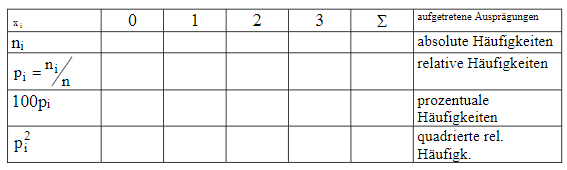
\includegraphics[width=\textwidth]{haeufigkeitstabelle-nominale-merkmale}
    \caption{Häufigkeitstabelle nominaler Merkmale}
    \label{fig:haeufigkeitstabelle-nominale-merkmale}
\end{figure}
\newline
Die Häufigkeitstabelle besteht aus $k$ Klassen bzw Kategorien. \newline
Aus der Tabelle kann man mehrere Sachen ablesen, die man ohnehin schon wusste:
\clm{Summe der absoluten Häufigkeiten}{}{Die absoluten Häufigkeiten, die der Tabelle ihren Namen geben, addierern sich zu $n$ (dem Stichprobenumfang)
\[\sum_{i=1}^{k} n_i = n\]
Beispiel: 3 Leute, davon 2 blond, einer dunkelhaarig. $2+1=3$.
}
\clm{Relative Häufigkeiten aus absoluten Häufigkeiten}{}{Dividiert man die absoluten Häufigkeiten durch $n$, erhält man die relativen Häufigkeiten. Damit kann man Stichproben mit verschiedenen Umfängen vergleichen. Die relativen Häufigkeiten addieren sich zu 1:
\[\frac{1}{n}\sum_{i=1}^{k} n_i = \sum_{i=1}^{k} p_i = 1\]
}
Um eine Idee von der Streuung der Daten zu bekommen, wird ein Maß eingeführt, welches man den \textbf{Index of Diversity} nennt:
\dfn{Index of Diversity}{
\[D = 1 - \sum_{i=1}^{k} p_i^2\]
Der Index of Diversity liegt in einem Wertebereich $0 \leq D < 1$.
Ein Wert von 0 bedeutet, dass alle Merkmalsausprägungen identisch sind (keine Vielfalt), während ein Wert nahe 1 auf eine hohe Vielfalt in der Verteilung der Merkmalsausprägungen hindeutet.
Es ist ratsam, den Wert $D$ nicht an 1, sondern an $1- k^{-1}$ zu vergleichen, weil k in den seltensten Fällen unendlich groß sein wird.
}

\subsection{Ordinalskalierte Merkmale}
Ordinalskalierte Werte sind Werte, die eine klare Hierarchie aufweisen, wobei die Abstände zwischen den Werten nicht gleich interpretiert werden können.
\begin{figure}[h]
    \centering
    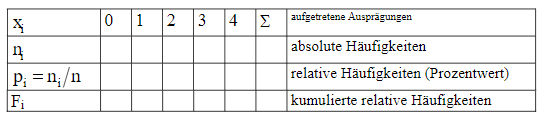
\includegraphics[width=\textwidth]{haeufigkeitstabelle-ordinale-merkmale}
    \caption{Häufigkeitstabelle ordinaler Merkmale}
    \label{fig:haeufigkeitstabelle-ordinale-merkmale}
\end{figure}
\newline
Das einzig Neue in dieser Tabelle (\ref{fig:haeufigkeitstabelle-ordinale-merkmale}) sind die \textbf{kumulierten relativen Häufigkeiten} (auch Summenhäufigkeiten).
Diese sind vor allem interessant, weil sie Vergleiche zwischen Stichproben unterschiedlicher Umfänge erlauben.
Dies ist aufgrund der eindeutigen Ordnung der Werte möglich.
\dfn{Kumulierte relative Häufigkeit}{
$F(x_i)$ stellt den Anteil der Werte dar, die höchstens die Merkmalsausprägung $x_i$ aufweisen.
\[F(x_i) = F_i = A(X \leq x_i) = \sum_{j=1}^{i} p_j \]
Üblicherweise wird die Summenhäufigkeit als Treppenfunktion dargestellt.
}
\newline
Übliche Kennwerte sind die \textbf{Quantile} (oder Prozentpunkte).
Die repräsentieren bestimmte Punkte einer Verteilung und teilen eben diese, basierend auf den kumulierten relativen Häufigkeiten, in gleich große Abschnitte ein. \newline
\dfn{Quantile}{
Quantile $X_w$ werden als die erste Merkmalsausprägung definiert, für welche die kumulierte relative Häfigkeit größer gleich $w$ ist.
\[F_i \geq w\]
Dies bedeutet, dass sie den Punkt in der Verteilung angeben, an dem mindestens ein bestimmter Prozentsatz $w$ der Daten erreicht oder überschritten wird.
}
\clm{Quartile}{}{
Zu den wichtigsten Quantilen gehören die Quartile.
Sie werden als $Q_i$ mit $i\in {1,2,3}$ angegeben.
Man spricht dann von dem ersten, zweiten oder dritten Quartil.
Die Quartile teilen die Rangwertreihe in 4 gleichmäßige Abschnitte auf und trennen bei 25\%, 50\% und 75\%.
}
Der \textbf{Median} ist ein bekanntes Beispiel für ein Quantil.
Er ist der Wert, bei dem die kumulierte relative Häufigkeit erstmals 50\% erreicht oder überschreitet.
Das bedeutet, dass 50\% der Daten kleiner oder gleich dem Median sind, während die anderen 50\% der Daten größer oder gleich dem Median sind.
Der Median ist somit $Q_2$ und berechnet sich als mittelster Wert der sortierten Liste, wenn die Anzahl der ungerade ist und als Mittelwert der beiden mittleren Werte, wenn die Anzahl gerade ist.


\subsection{Streuungsmaße}
\begin{itemize}
    \item Die \textbf{Spann- oder Streuweite} $R$ (wie Range) ist die Differenz zwischen den Extremwerten:
    \[R = x^{max} - x^{min}\]
    Die Streuweite wird üblicherweise zusammen mit dem Mittelwert angegeben, weil sie andernfalls nicht mehr aussagekräftigt wäre.
    \item Der \textbf{Interquartilsabstand} $IQA$ gibt den Bereich an, der von den mittleren 50\% der Werte bedeckt wird.
    \[IQA = Q_3 - Q_1\]
    \item Der \textbf{relative Quartilsabstand} berechnet sich aus dem Verhältnis von $IQA$ und $R$.
    Je näher diese Zahl an 1 ist, desto gestreuter ist die Verteilung.
    Je näher diese Zahl an 0 ist, desto konzentrierter ist die Verteilung.
    \[IQA_r = \frac{IQA}{R}\]
    \item Der \textbf{mittlere Quartilsabstand} $MQA$ wird als die Hälfte des $IQA$ definiert.
    \[MQA = \frac{IQA}{2} = \frac{Q_3 - Q_1}{2}\]
    Bei symmetrischen Verteilungen gilt entsprechend mit $Md$ als Median:
    \[MQA = \frac{Q_3 - Q_1}{2} = Q_3 - Md\]
\end{itemize}


